\chapter{Optimization Strategies \label{ch:optstrat}}

\section{The Generalized Optimization Loop}

In Mesquite a generalization of the optimization strategy is used to implement a wide variety of optimization strategies.  Before discussing the different types of optimization strategies that can be implemented with Mesquite we will first need to discuss the generalized strategy.

The mesh can be decomposed into subsets called {\em patches}.  The specifics of this mesh decomposition are discussed in Section \ref{sec:patches}.  The optimization is done by repeatedly iterating over the set of patches, optimizing each separately.

\begin{figure}[htb!]
\begin{center}
\noindent\makebox[\textwidth]{%
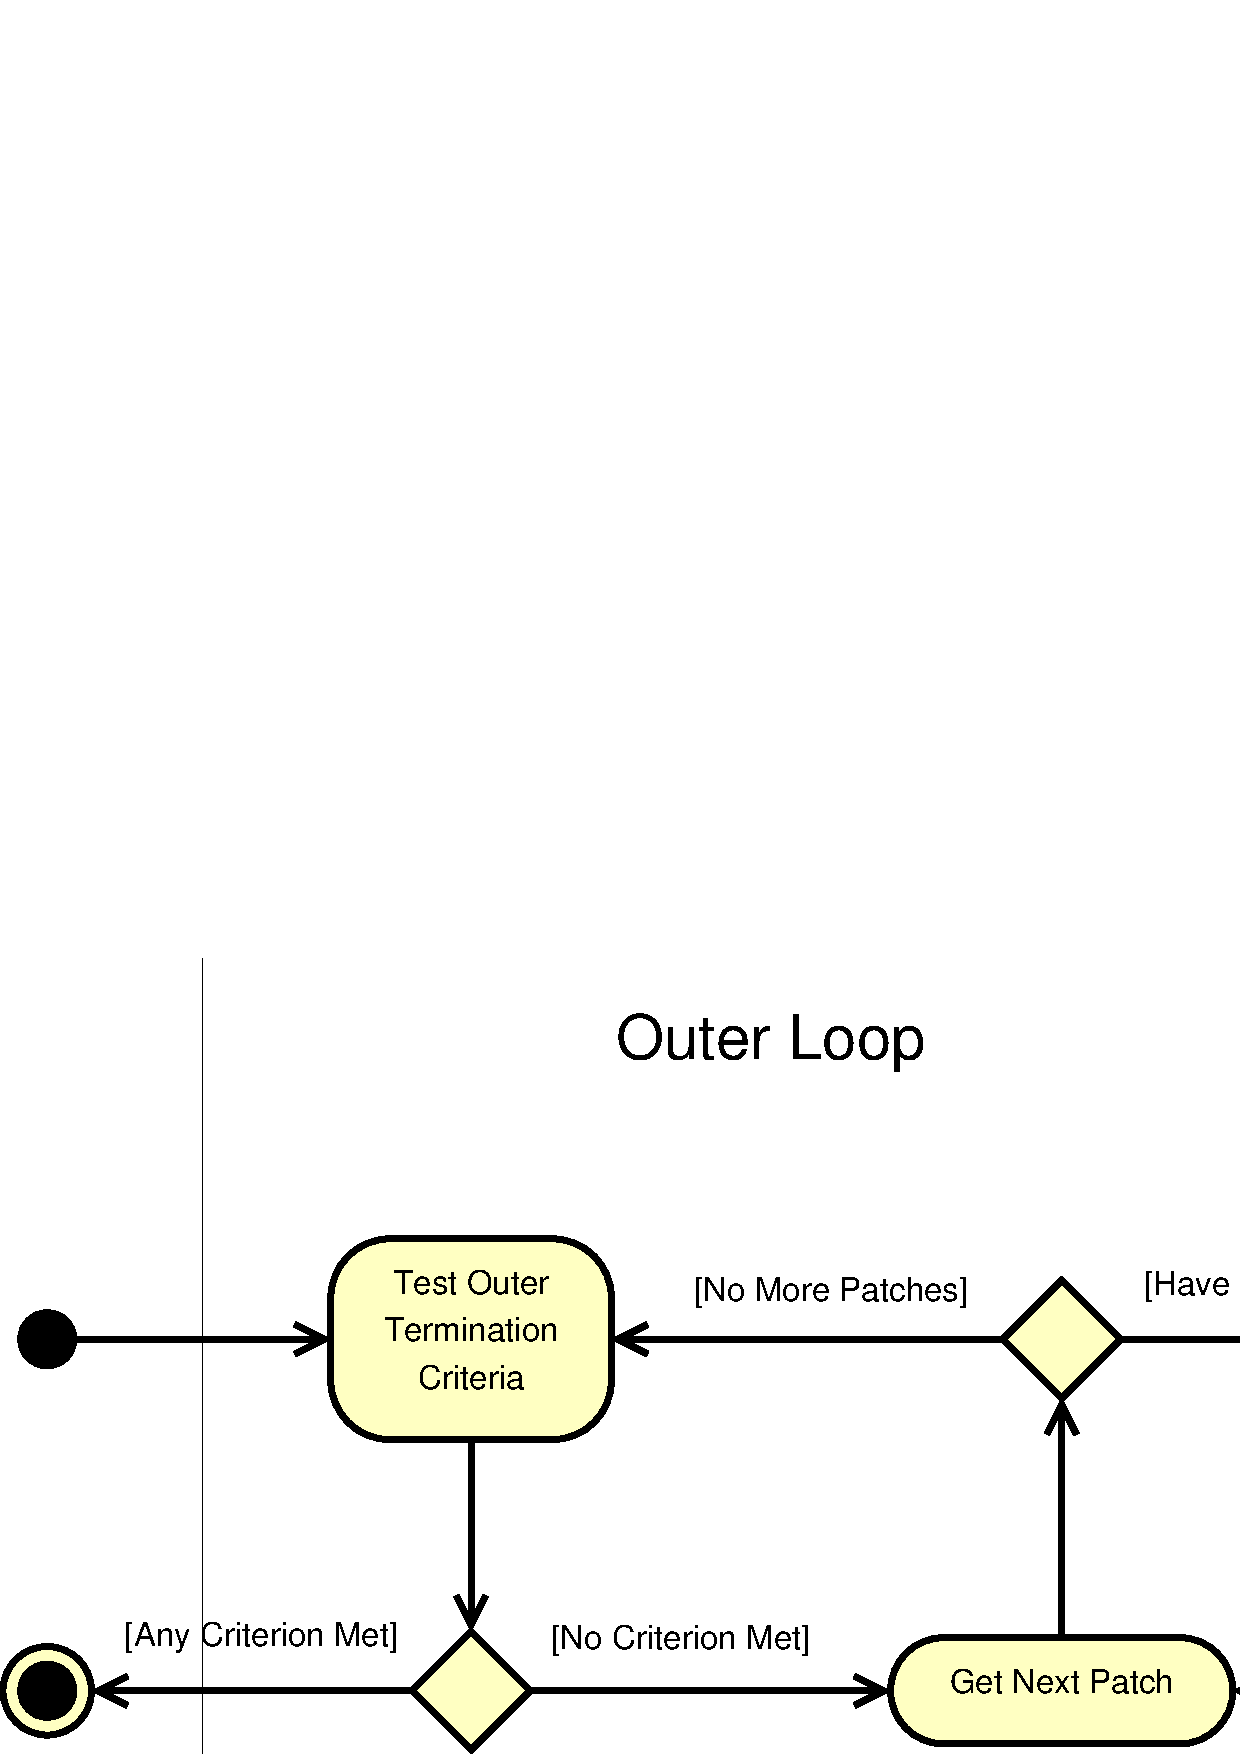
\includegraphics[width=6.5in]{generalized_optimization}}
\caption{\em Optimization Loop \label{fig:genoptloop}}
\end{center}
\end{figure}

Figure \ref{fig:genoptloop} depicts the generalization of optimization strategies in Mesquite.  The generalized optimization is composed of three loops shown as non-overlapping square cycles in the diagram.  The test to exit each loop is performed at the decision points (diamonds) in the diagram.  The loops are logically nested from left to right, such that the right most loop is performed within a single iteration of the loop to the left of it.  The inner- and outer-most loops terminate based on user-definable termination criterion.  The center loop is the iteration over the set of patches composing the mesh.

The inner-most loop (the right-most cycle in the diagram) represents the iterative optimization of the mesh contained in a single patch.  This optimization is done until the {\em inner termination criterion} is met.  Once the inner criterion is met the optimizer advances to the next patch and the inner loop is entered again to optimize that patch.  Once each patch has been optimized the {\em outer termination criterion} is tested.  If the criterion has not been met then the loop over the set of patches is repeated.

The set of outer termination criteria determine when the optimization of the entire mesh is complete.  The set of inner termination criteria determine when the optimization of a single patch is complete.  Both sets of criteria are tested before entering their respective loops.  If a criterion is met before the loop starts then no iterations of the corresponding loop will be performed.

The outer loop(s) are implemented in the {\texttt VertexMover} class.  The inner loop is implemented in subclasses.  The {\texttt LaplacianSmoother} class in Mesquite provides a traditional Laplace smoother.  For this class the mesh is decomposed into patches that each contain a single free vertex and the adjacent elements, one patch for each free vertex in the mesh.  For Laplace smoothing the inner (per-vertex) optimization is not iterative.  The inner loop always has an implicit termination criterion of a single iteration.  Any other inner termination criterion will still be tested before performing the relaxation of the free vertex in the patch such that if any such criterion is met no optimization of the vertex will be performed.  However, culling (Section \ref{sec:culling} can have a similar effect while typically producing better results.  Passes are made over the entire mesh until one of the specified outer termination criterion is met.

\section{Patches \label{sec:patches}}


Mesquite can operate on a decomposition of the mesh into subsets called {\em patches}.  Each patch is optimized individually.  The overall mesh optimization is performed by repeatedly iterating over the set of patches.  Mesquite provides two build-in mesh decompositions\footnote{Mesquite includes an additional decomposition of the mesh into single-element patches which is not suitable for use in optimization.  It is used internally for quality assessment and other purposes}: element-on-vertex patches and a global patch.  

\begin{figure}[htb]
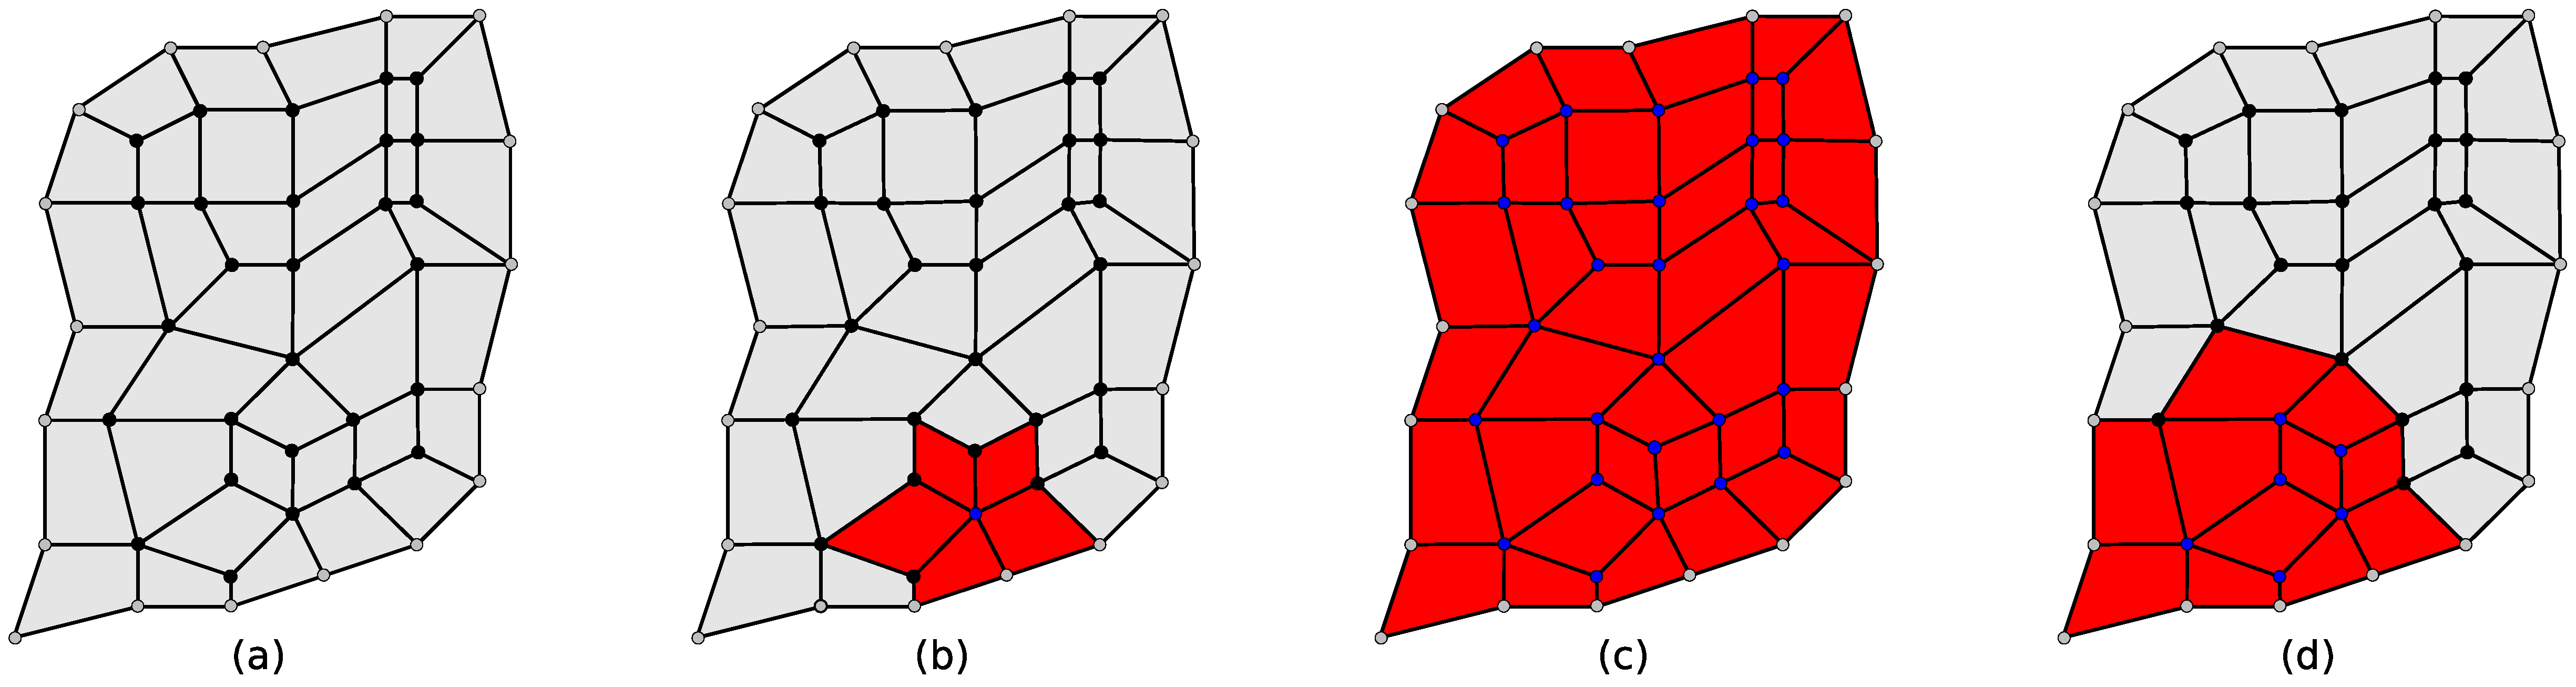
\includegraphics[width=5in]{patches-horiz}
\caption{Miscellaneous patch configurations.\label{fig:patch-types}}
\end{figure}

The global patch is a ``decomposition'' where the entire mesh is contained in a single patch.  This is used in the global optimization strategy discussed in Section \ref{sec:global}. Figure \ref{fig:patch-types}c illustrates the global patch.

The element-on-vertex decomposition subdivides the mesh into a single patch for each free vertex.  Each patch includes the layer of elements adjacent to the free vertex.  A element-on-vertex patch is illustrated in Figure \ref{fig:patch-types}b.  This decomposition is typically used for all optimization strategies discussed in this chapter except for global optimization.  Any other decomposition except global may be used for any of the optimization strategies.  All of the discussed strategies other than global do not make sense for a global patch.

Any patch decomposition can be used with Mesquite.  While no other decomposition strategy is provided with Mesquite, the any implementation of the {\texttt PatchSet} interface can be associated with any quality improver that supports it (any subclass of {\texttt PatchSetUser}, currently all except {\texttt LaplacianSmoother}).  An implementation of that interface is expected to provide three things:
\begin{enumerate}
\item An enumeration of all the patches in the decomposition of the mesh
\item For each patch, the set of vertices to optimize
\item For each patch, the set of elements for which the quality is to be optimized (typically all elements containing the vertices to be optimized.)
\end{enumerate}
A normal decomposition will be done such that each free vertex in the mesh is optimized in exactly one patch, but Mesquite does not enforce this.  Having a free vertex be optimized in no patch will result in that vertex effectively being fixed for the optimization.  A decomposition that optimized the same vertices in multiple patches is allowable, and should have no adverse side effects unless doing a Jacobi optimization (Section \ref{sec:jacobi}).

The listing below shows how a custom implementation of the {\texttt PatchSet} interface can be used with the {\texttt SteepestDescent} solver.

\begin{lstlisting}[frame=single]
MyMeshDecomposition my_patch_set;
SteepestDescent quality_improver( &objective_function );
\<quality_improver.use_patch_set(&my_patch_set);\>
\end{lstlisting}

In any of the examples later in this chapter that call {\texttt use\_element\_on\_vertex\_patch()}, that call may be sustitued with a call to {\texttt use\_patch\_set} to use some decomposition other than single-vertex patches.

\section{Global \label{sec:global}}

For a global optimization an objective function that measues the quality of the mesh is minimized using a numerical solver.  The coordinates of all of the free vertices in the mesh are the free variables in the optimization.  This is the default mode of operation for most solver-based implementations of the {\texttt QualityImprover} interface.

A global optimization is simplest form of the generalized optimization loop.  In this mode the mesh is ``decomposed'' into a single patch containing the entire mesh.  The outer loops in Figure \ref{fig:genoptloop} are executed only once.  The entire optimization process happens in the inner loop.  For global optimization the outer termination criterion is the default of a single iteration.  The inner termination criterion should be used to terminate the optimization process.  Setting some other outer termination criterion is not prohibited, but will result in a much less efficient optimization process.  There is no logical difference between inner and outer termination criterion, but each iteration of the outer loop begins with a clean solver state which will result in less efficient operation of the solver.  Even steepest descent, the simplest solver, caculates a initial step size based on the previous iteration of the inner loop.  

The listing below shows how global optimization can be selected.

\begin{lstlisting}[frame=single]
// Create global optmizer instance
SteepestDescent improver( &objective_function );
\<improver.use_global_patch();\>

// Set only inner termnation criterion for 
// global optimization
TerminationCriterion inner;
inner.add_absolute_vertex_movement( 1e-3 );
improver.set_inner_termination_criterion( &inner );

// Run optimization
InstructionQueue queue;
queue.set_master_quality_improver( &improver, err );
queue.run_instructions( &mesh, err );
\end{lstlisting}

\section{Nash Game \label{sec:nash} }


\begin{lstlisting}[frame=single]
// Create Nash optmizer instance
SteepestDescent improver( &objective_function );
\<improver.use_element_on_vertex_patch();\>

// Set inner and outer termnation criterion for 
// non-global patch
TerminationCriterion inner, outer;
outer.add_absolute_vertex_movement( 1e-3 );
inner.add_iteration_limit( 2 );
improver.set_outer_termination_criterion( &outer );
improver.set_inner_termination_criterion( &inner );

// Run optimization
InstructionQueue queue;
queue.set_master_quality_improver( &improver, err );
queue.run_instructions( &mesh, err );
\end{lstlisting}


\section{Block Coordinate Descent \label{sec:bcd} }

\begin{lstlisting}[frame=single]
// Create BCD optmizer instance
SteepestDescent improver( &objective_function );
improver.use_element_on_vertex_patch();
\<improver.do_block_coordinate_descent_optimization();\>

// Set inner and outer termnation criterion for 
// non-global patch
TerminationCriterion inner, outer;
outer.add_relative_quality_improvement( 1e-2 );
inner.add_iteration_limit( 2 );
improver.set_outer_termination_criterion( &outer );
improver.set_inner_termination_criterion( &inner );

// Run optimization
InstructionQueue queue;
queue.set_master_quality_improver( &improver, err );
queue.run_instructions( &mesh, err );
\end{lstlisting}


\section{Culling \label{sec:culling}}


\begin{lstlisting}[frame=single]
// Create Nash optmizer with culling
SteepestDescent improver( &objective_function );
improver.use_element_on_vertex_patch();

// The culling criterion is effectively an outer 
// termination criterion because optimization will 
// always stop when all patches are culled.  We 
// must explicitly pass an empty outer termination 
// criterion to replace the default of one iteration.
// Additional outer termination criteria may also be 
// specifed.
TerminationCriterion inner, outer;
\<inner.cull_on_absolute_vertex_movement( 1e-3 );\>
inner.add_iteration_limit( 2 );
improver.set_outer_termination_criterion( &outer );
improver.set_inner_termination_criterion( &inner );

// Run optimization
InstructionQueue queue;
queue.set_master_quality_improver( &improver, err );
queue.run_instructions( &mesh, err );
\end{lstlisting}

\section{Jacobi \label{sec:jacobi}}

\begin{lstlisting}[frame=single]
// Create Jacobi optmizer instance
SteepestDescent improver( &objective_function );
improver.use_element_on_vertex_patch();
\<improver.do_jacobi_optimization();\>

// Set inner and outer termnation criterion for 
// non-global patch
TerminationCriterion inner, outer;
outer.add_absolute_vertex_movement( 1e-3 );
inner.add_iteration_limit( 2 );
improver.set_outer_termination_criterion( &outer );
improver.set_inner_termination_criterion( &inner );

// Run optimization
InstructionQueue queue;
queue.set_master_quality_improver( &improver, err );
queue.run_instructions( &mesh, err );
\end{lstlisting}
